
\chapter{Discussion}\label{c4}

As mentioned earlier, kNN compares the test sample to k neighbouring training samples to determine the class. This means all training samples have to be stored in memory \cite{Gutie} which in turn could slow down the computer, causing the classifier to take a longer time to produce results. Being a non-parametric technique \cite{16N} unlike DT and RF, kNN is prone to the curse of dimensionality \cite{Gutie}, which happens when the dimensions or number of features increases \cite{Distr}. This might explain the lower performance metric scores in comparison. There are big differences between the optimal k values for some turbines as shown in Figure~\ref{f3} which could be due to the data for each turbine having different distributions and characteristics.

Overall, using a single multiclass-multilabel classifier with imbalanced training data produced better scores, which could be due to presence of correlations between the different turbine categories used as labels that are generalised better using this approach \cite{110}.

As the labels `gearbox' and `electrical system' are in the top three out of 14 labels used causing longest downtimes, they should have more samples classed as `faulty' and `X hours before fault' compared to other categories, which therefore should result in better performance as the classifier would have learned the characteristics of different samples belonging to the same classes. This was not the case, however, looking at the confusion matrices in Appendix~\ref{a4}. The classifier tends to misclassify `faulty' and `X hours before fault' classes as `normal' at a higher rate than the accuracy for these classes. This is still the case after removing the `curtailment' class, which saw an improvement in the accuracy of the `faulty' class. The accuracies of `X hours before fault' classes could potentially be increased by reducing the 6-hour intervals used and the maximum of 48 hours before a fault. The analysis should be repeated by reducing 48 hours to a smaller timescale, such as 12 hours, or by combining all samples that fall under this with `faulty' points to make the classification binary. Although this is likely to improve the performance, the classifier will not be able to give an indication of the timescale before a potential fault, therefore making it more difficult to decide on the appropriate action to be taken to avoid catastrophic failure in the turbine.

Based on the feature importance in Table~\ref{t6}, active power SCADA fields were least influential in predicting faults for both labels. The labelled power curves for `electrical system' in Figure~\ref{f5} below shows no clear relationship between fault points and the power curve shape. There are also many overlapping `normal', `faulty' and `X hours before fault' points even after filtration of curtailment and anomalies, which could explain why this feature was less important.

\begin{figure}
    \centering
    \begin{subfigure}[t]{.5\textwidth}
        \centering
        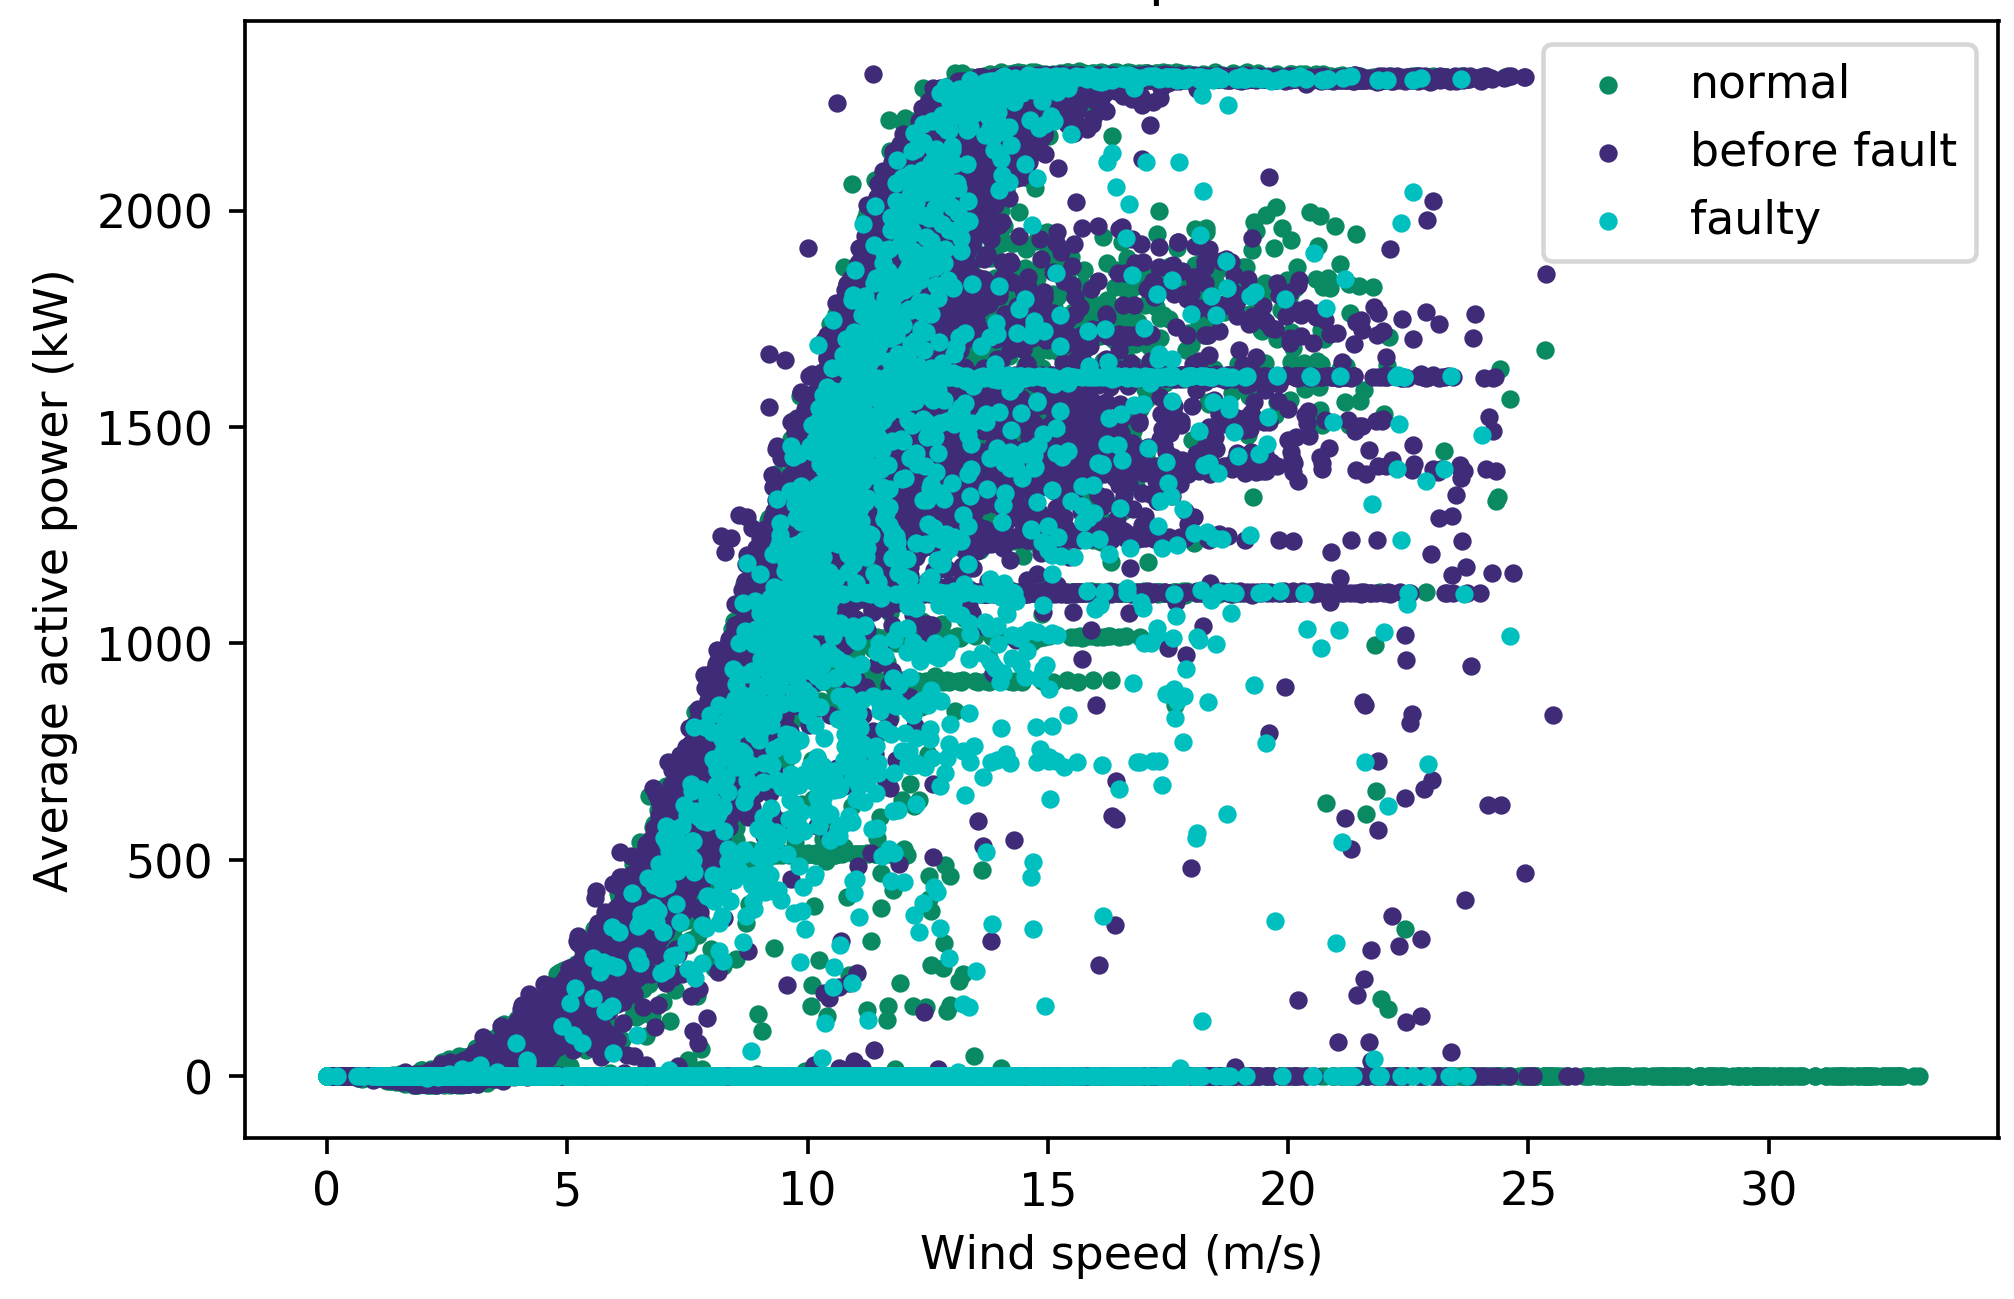
\includegraphics[height=5cm]{f5a}
        \caption{\label{f5a}}
    \end{subfigure}%
    \begin{subfigure}[t]{.5\textwidth}
        \centering
        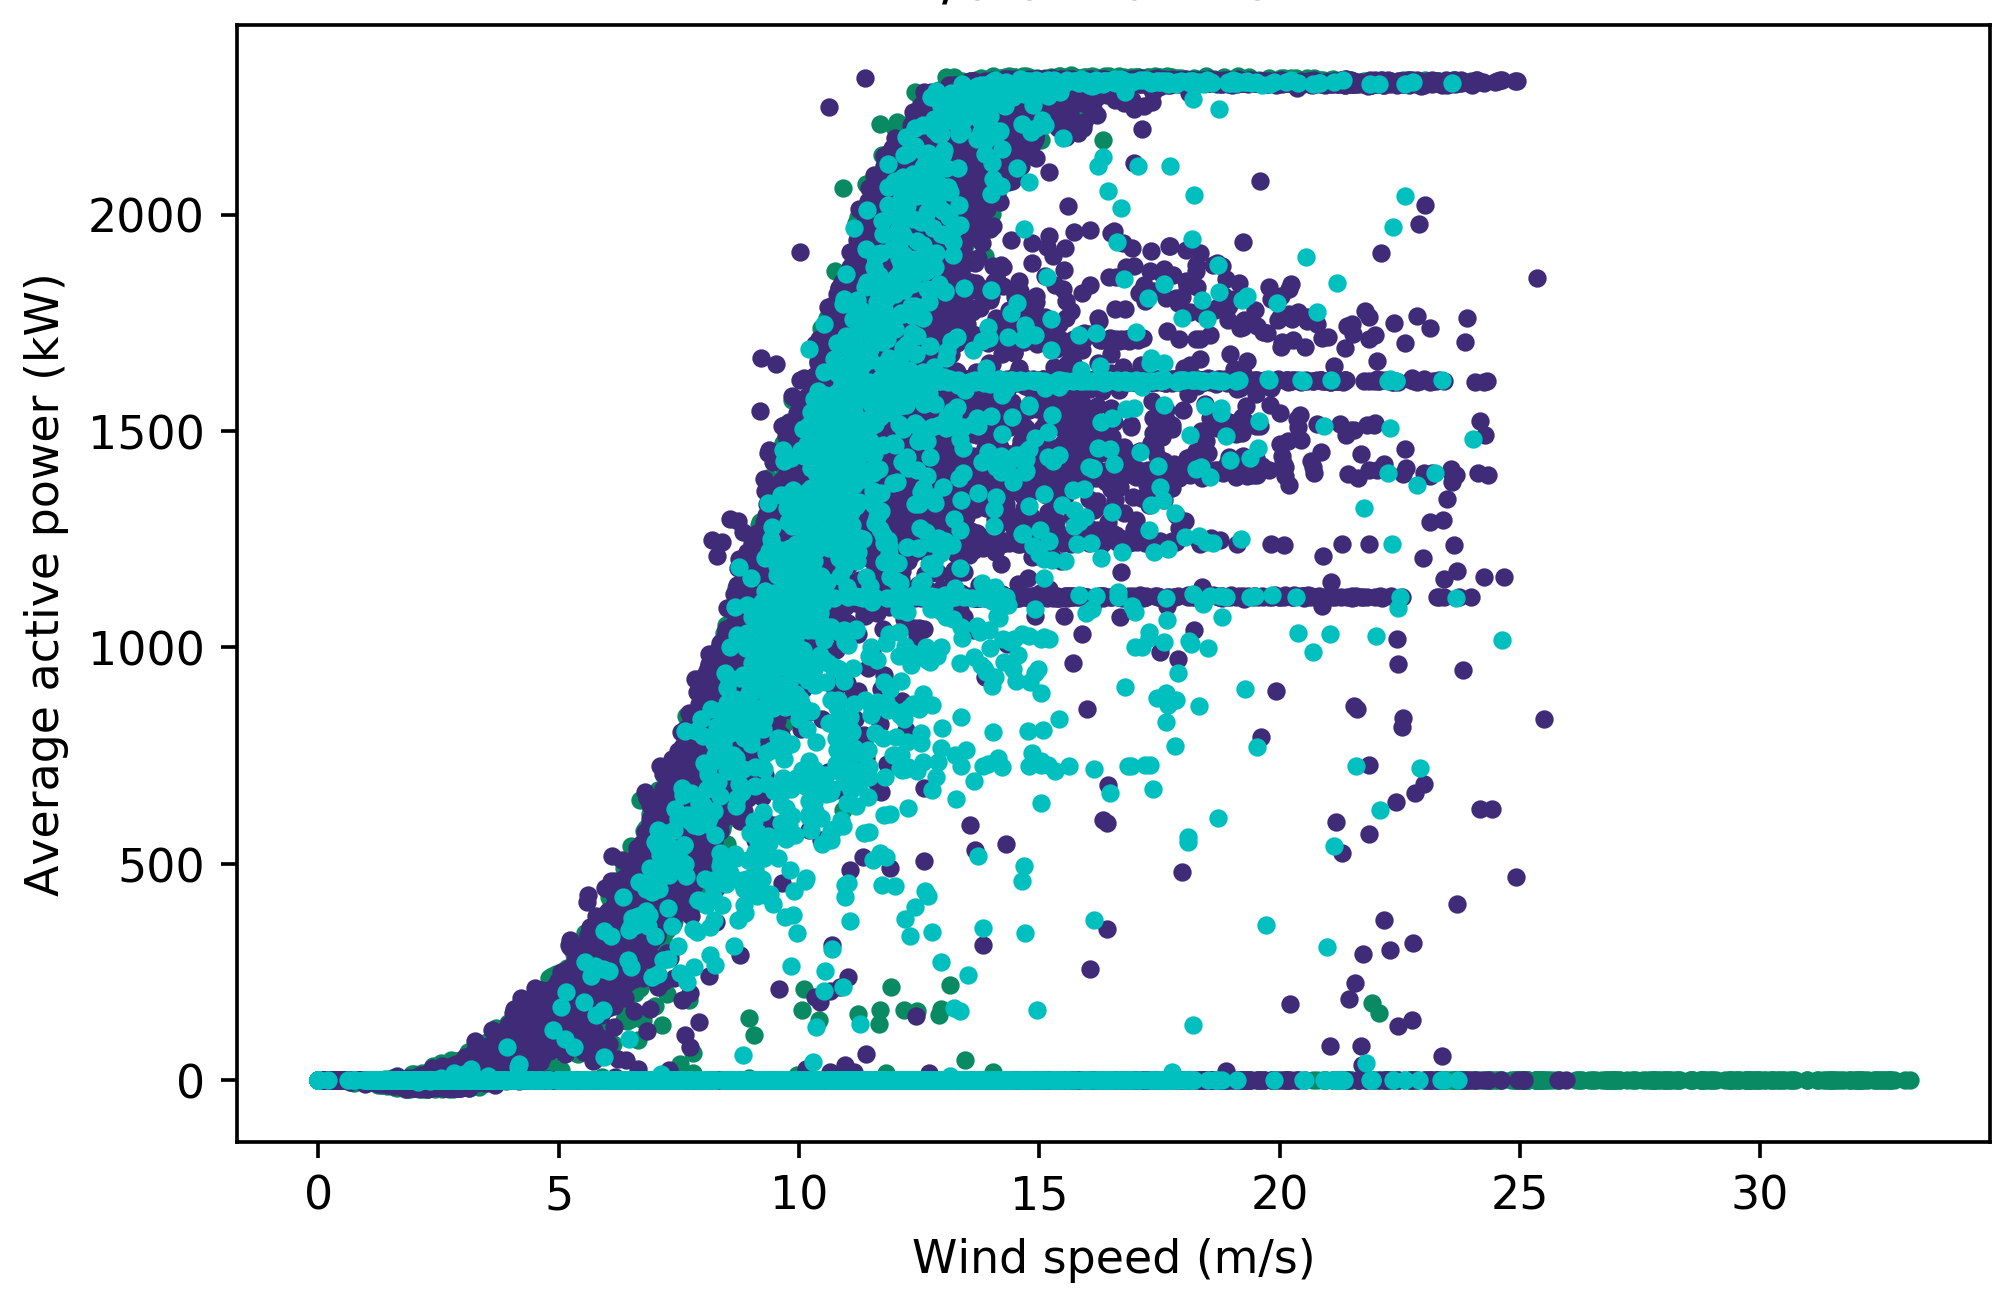
\includegraphics[height=5cm]{f5b}
        \caption{\label{f5b}}
    \end{subfigure}
    \begin{subfigure}[t]{.5\textwidth}
        \centering
        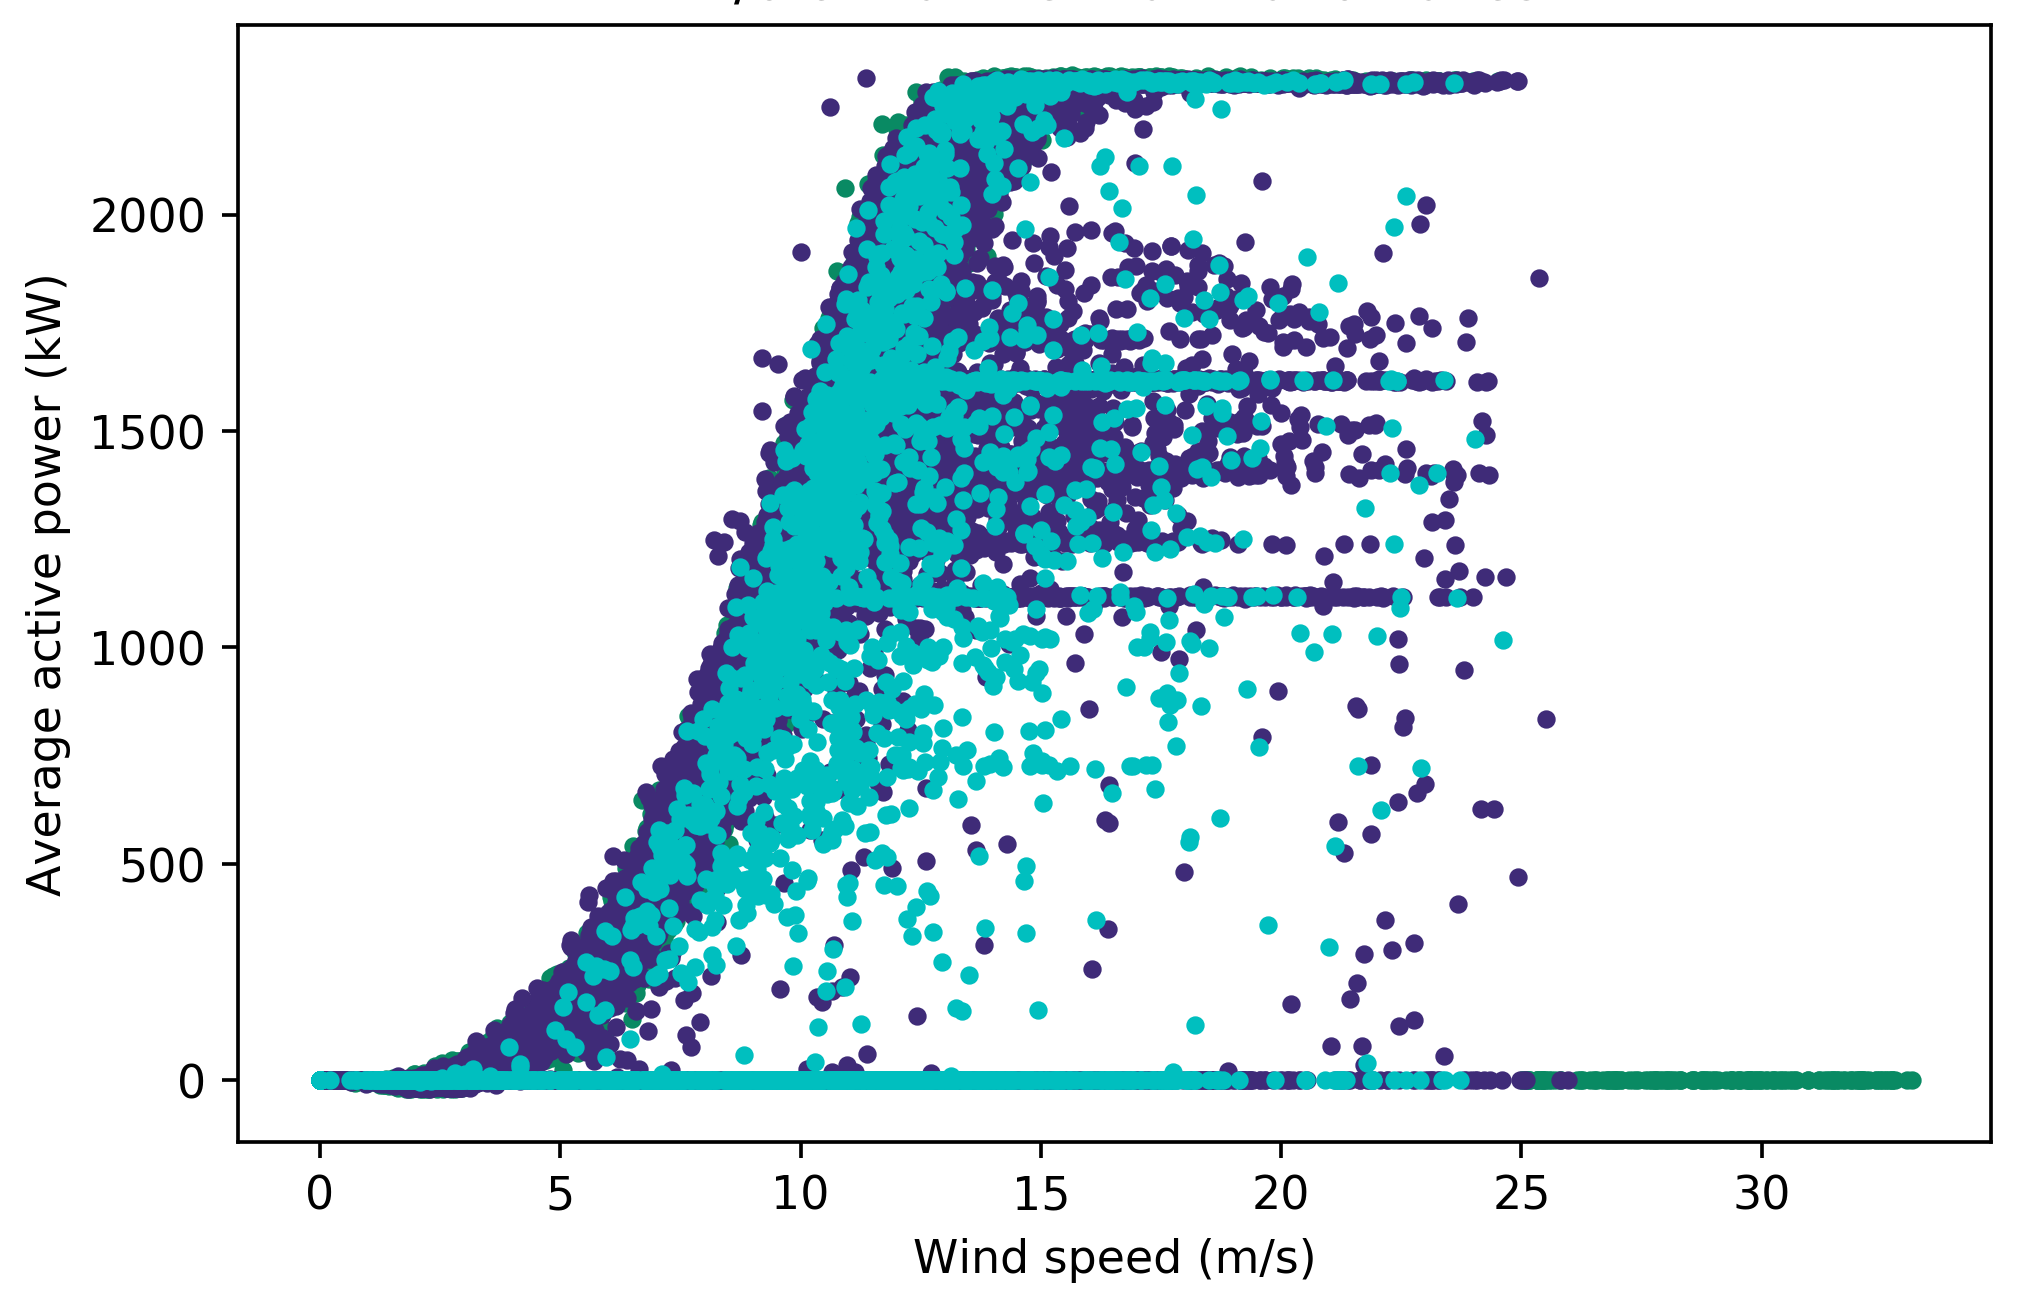
\includegraphics[height=5cm]{f5c}
        \caption{\label{f5c}}
    \end{subfigure}
    \caption{\label{f5}Labelled power curve for turbine 1 with turbine category 10 (`electrical system') through the two stages of filtering out anomalous and curtailment points labelled as `normal'. The original power curve is shown in \ref{f5a}. The first stage involves a filter based on a pitch angle threshold, which produces \ref{f5b}. The second stage involves several additional filters to produce the final power curve \ref{f5c}.}
\end{figure}

The reactive power and generator speed played a bigger role in the classification for `electrical system', which makes sense considering the reactive power is produced as a result of impedance in the current due to electromagnetic fields produced by generators and transformers \cite{React}. It is likely that the features used in classification for this label are unsuitable. A fault in the electrical system would be reflected in voltages, currents, frequencies \cite{Overb} and temperature of power switchboards and cables. Electrical system faults could also be caused by environmental conditions such as lightning strikes and contact of wires with wildlife \cite{Overb}. If there are such conditions recorded as environmental downtime categories, these should be accounted for when analysing faults in the electrical system.

The `gearbox' label was also found to perform poorly for these classes, despite having a higher mean F1 score than `electrical faults', which could be due to feature selection as well. Statistics from the National Renewable Energy Laboratory's gearbox failure database indicate that most faults are caused by bearings, gears and other components including filtration and lubrication systems \cite{Stati15}. These are mostly due to wear, fatigue and cracks \cite{Sheng11} and may be detected with higher accuracy if the features include quantities such as torque, oil pressure and gearbox temperature.

The SCADA data provided for this project only had 17 SCADA fields, of which 10 are used as features. This did not include voltages, currents, frequencies, torques or temperature readings, but the SCADA system for the turbine model used does measure these parameters. When a more complete SCADA data is available, the evaluation should be done by increasing the number of features to include these fields. The role of environmental conditions on failures could explain why wind speed and direction were very influential in detecting faults in the two labels analysed, although further in-depth analysis is required to verify this.

Balancing the training dataset improved the classification accuracy of `X hours before fault' classes slightly. An overall improved model may be developed by oversampling only these classes for training, but there is a trade-off between this and the training time and computational resources required.

The dataset could have incorrect readings in the SCADA fields caused by broken or unresponsive sensors which are not detected as unusual when the downtime data is used in labelling. This was why a power threshold before cut-in speed was applied to remove redundant data points, by visually inspecting the power curve of the turbine as seen in Figure~\ref{f1}. The dataset should be manually inspected for all other features using curves such as pitch versus power and power versus rotor speed, to see if there are any other incorrect values previously undetected which may affect the classifier's accuracy in detecting faults. The rows of data corresponding to these values should then be excluded from the training data.

\section{Future work}

In addition to possible areas for future work discussed above, the following were identified.

When more data is available, the analysis should be repeated using historic datasets spanning the life of the turbine. Historic data would have recorded the different states a turbine has experienced over its life, and therefore when a classifier is trained on this, it could detect future turbine states easier. However, this will mean the training data will be bigger, which in turn causes longer training time and more computing resources to be used. Another area of work is to test the performance of a classifier using different lengths of datasets for training while keeping the testing set and hyperparameter settings constant. This will allow for the most appropriate length of dataset for training to be determined based on the resources available to produce satisfactory results in terms of training time and classification accuracy.

After a classifier has been trained and used in practice, its performance over time should be monitored. If the performance is found to diminish over time or after a major component replacement, the classifier should be retrained using recent data. As the classification makes a distinction between the different faults, the ability to alert relevant maintenance professionals for a specific fault automatically is possible.

Instead of using turbine categories in the downtime data, which is supervised, for labelling, the alarm logs, which are unsupervised, can instead be used to compare the results. The number of alarm logs for the turbines used, however, is 480, compared to 23 turbine categories. This will mean the number of labels will be much higher, which will cause longer computational time. A solution to reduce this is to group similar alarms into one class. Another approach would be to use a single label with each alarm as a separate class, but there is likely to be overlap between classes when fault prediction is also included. If actual failure records are available, a comparison can be made between the predicted classes, actual classes, and actual failures that have occurred and their costs.

Further optimisation of hyperparameters is possible, such as finding the optimal number of estimators for RF. Each optimisation takes time and is limited by the specifications of the computer used, which is why this was not carried out in this project. Detailed analysis done on the results using RF for two labels above should be repeated for each label and classifier used for fair comparisons to be made.

The methodology could also be tested for wind turbines of different models in different sites. Provided these turbines have similar SCADA data with downtime records, only slight modifications to the codes, such as the data source, field names, and number of features, would be required in order to be used on other turbine models.

In industry, a cost function analysis needs to be done prior to implementing this fault detection method. It is defined as the cost of a false alarm (false positive) or failing to detect a fault in advance (false negative). False positives and false negatives both incur charges. The first is due to transporting labour and equipment to site, which could be expensive especially for sites in harsh environments, such as offshore wind farms. The second would cause unscheduled downtime, the loss of revenue due to no power generation and replacement of turbine components due to irreversible damage. This cost should then be compared to the cost of alternatively using a condition monitoring system, and the overall cost of running the wind farm or wind turbine. The analysis should give an indication on which performance metric is more important; if the cost of false negatives is more, attention should be paid to the recall score, while the precision is more important if false positives cost more \cite{deRu15}.
